\documentclass[a4paper,11pt]{article}
\usepackage{fullpage}

\usepackage[utf8]{inputenc}
\usepackage[british]{babel}

\usepackage{amsmath}
\usepackage{amssymb}
\usepackage{amsthm} \newtheorem{theorem}{Theorem}
\usepackage{color}
\usepackage{float}
\usepackage{listings}

\usepackage{multirow}
\usepackage{tikz} \usetikzlibrary{trees}
\usepackage{hyperref}  % should always be the last package


% useful (wrappers for) math symbols:
\newcommand{\Cardinality}[1]{\left\lvert#1\right\rvert}
%\newcommand{\Cardinality}[1]{\##1}
\newcommand{\Ceiling}[1]{\left\lceil#1\right\rceil}
\newcommand{\Floor}[1]{\left\lfloor#1\right\rfloor}
\newcommand{\Iff}{\Leftrightarrow}
\newcommand{\Implies}{\Rightarrow}
\newcommand{\Intersect}{\cap}
\newcommand{\Sequence}[1]{\left[#1\right]}
\newcommand{\Set}[1]{\left\{#1\right\}}
\newcommand{\SetComp}[2]{\Set{#1\SuchThat#2}}
\newcommand{\SuchThat}{\mid}
\newcommand{\Tuple}[1]{\langle#1\rangle}
\newcommand{\Union}{\cup}
\newcommand{\Returns}{\longrightarrow}


\title{\textbf{Algorithms \& Data Structures II (course 1DL231) \\
    Uppsala University -- Autumn 2014 \\
    Report for Assignment $n$  % replace n by 1, 2, or 3,
    by Group $t$}}              % replace t by your group number/name

\author{Clara CLEVER \and Whiz KIDD}  % replace by your name(s)

%\date{Month Day, Year}
\date{\today}



\begin{document}

\maketitle

\noindent
This document shows the ingredients of a good homework report for the AD2 course.  The \LaTeX\ source code of this document exemplifies almost everything you need to know about \LaTeX\ in order to typeset a professional-looking assignment report (for the AD2 course).  Use it as a starting point for imitation and delete everything irrelevant.
The usage of \LaTeX\ is \emph{optional}, but highly recommended, for reasons that will soon become clear to those who have never used it before; any learning time is \emph{outside} the budget of this course, but will hugely pay off, if not in this course then in the next course(s) you take and when writing your BSc, MSc, or PhD thesis.

\section{Insertion Sort}
\label{sect:isort}

Insertion sort is an efficient algorithm for sorting a small number of
elements.  Insertion sort works the way many people sort a hand of
playing cards.  We start with a empty left hand and the cards face
down on the table.  We then remove one card at a time from the table
and insert it into the correct position in the left hand.  To find the
correct position for a card, we compare it with each of the cards
already in the hand, from right to left, as illustrated in.  At all times, the cards held in the left hand
are sorted, and these cards were originally the top cards of the pile
on the table.  

\subsection{Specification and Program}
\label{sect:pgm:isort}


\subsection{Analysis}
\label{sect:analysis:isort}

\begin{equation*}
  T(n) =
  \begin{cases}
    \Theta(1) & \text{if~} n < 2 \\
    T(n-1) + T_{\text{ins}}(n) & \text{if~} n \geq 2
  \end{cases}
\end{equation*}
Using recurrence~(), we get the following time complexity
results:

\begin{theorem}
  \label{thm:ind}
  The following recurrence, for some \emph{constants} $a$ and $b$:
  \[
  T(n) =
  \begin{cases}
    \Theta(1) & \text{if~} n < b \\
    a \cdot T(n-1) + \Theta(1) & \text{if~} n \geq b
  \end{cases}
  \]
  has $\Theta(n)$ as closed form for $a = 1$, and $\Theta(a^n)$ as
  closed form for $a > 1$.
\end{theorem}

\begin{proof}
  By induction (left as an exercise to the reader in the AD1 course).
\end{proof}

\section*{Intellectual Property}

We certify that the material in this report is solely produced by its
authors, except where otherwise indicated and clearly referenced.

\bibliographystyle{abbrv}
\bibliography{algorithms}

% cut everything below here until the \end{document} line before submitting

\newpage
\section*{Checklist before Submitting}

In order to protect yourself against an unnecessary loss of points,
and in order to show both self-respect and respect for the human
reader of your report, please use the following checklist before
submitting:
\begin{itemize}
\item Crosscheck your report against the homework instructions.
\item Crosscheck against the technical writing and \LaTeX\ advice
  below.  The style manual and checklist at
  \url{http://www.it.uu.se/research/group/astra/checkList.pdf} offers
  many further pieces of advice.  Common errors in English usage are
  discussed at \url{http://public.wsu.edu/~brians/errors/errors.html}.
  In particular, common errors in English usage by native Swedish
  speakers are listed at
  \url{http://www.cb.uu.se/~cris/English_language.html}.
\item Spellcheck all documents, including the comments in the source
  code.
\item Proofread, if not grammar-check, your report at least once per
  teammate.
\end{itemize}

\section{More \LaTeX\ and Technical Writing Advice}

Unnumbered itemisation (only to be used when the order of the items
does \emph{not} matter):\footnote{Use footnotes very sparingly, and
  remember that footnote pointers are never preceded by a space and
  always glued immediately \emph{behind} the punctuation, if there is
  any.}
\begin{itemize}
\item Unnumbered displayed formula:
  \[
  E = m \cdot c^2
  \]
\item Numbered displayed formula (which is normally cross-referenced
  somewhere):
  \begin{equation}
    \label{eq:emc2}
    E = m \cdot c^2
  \end{equation}
\item Formula --- the same as formula~(\ref{eq:emc2}) --- spanning
  more than one line:
  \begin{gather*}
    E \\ = \\ m \cdot c^2
  \end{gather*}  
\end{itemize}
Numbered itemisation (only to be used when the order of the items
\emph{does} matter):
\begin{enumerate}
\item First do this.
\item\label{item:that} Then do that.
\item If we are not finished, then go back to Step~\ref{item:that},
  else stop.
\end{enumerate}

The typesetting of tables and elementary mathematics is exemplified in
Table~\ref{tab:maths}; see
\url{ftp://ftp.ams.org/pub/tex/doc/amsmath/short-math-guide.pdf} for
many more details.

Do \emph{not} use programming-language-specific lower-ASCII notation
(such as $!$ for negation, $\&\&$ for conjunction, $||$ for
disjunction, and the equality sign $=$ for assignment) in algorithms
or formulas (but rather $\neg$ or $\mathbf{not}$, $\land$ or $\&$ or
$\mathbf{and}$, $\lor$ or $\mathbf{or}$, and $\gets$ or $:=$,
respectively), as this testifies to a very strong confusion of
concepts.

\begin{table}[t]  % make it float to the top of a page
  \centering
  \begin{tabular}{|r|l|c|}  % right left centre
    \hline
    Topic & \LaTeX\ code & Appearance \\ \hline
    \hline
    Greek letter & \verb|$\Theta,\Omega,\epsilon$| & $\Theta,\Omega,\epsilon$ \\ \hline
    multiplication & \verb|$m \cdot n$| & $m \cdot n$ \\ \hline
    division & \verb|$\frac{m}{n}, m \div n$| & $\frac{m}{n}, m \div n$ \\[+2pt] \hline
    rounding down & \verb|$\lfloor n \rfloor$| & $\lfloor n \rfloor$ \\[+2pt] \hline
    rounding up & \verb|$\lceil n \rceil$| & $\lceil n \rceil$ \\[+2pt] \hline
    binary modulus & \verb|$m \bmod n$| & $m \bmod n$ \\ \hline
    unary modulus & \verb|$m = n \mod \ell$| & $m = n \mod \ell$ \\ \hline
    root & \verb|$\sqrt{n},\sqrt[3]{n}$| & $\sqrt{n},\sqrt[3]{n}$ \\ \hline
    exponentiation, superscript & \verb|$n^{i}$| & $n^{i}$ \\ \hline
    subscript & \verb|$n_{i}$| & $n_{i}$ \\ \hline
    overline & \verb|$\overline{n}$| & $\overline{n}$ \\ \hline
    base $2$ logarithm & \verb|$\lg n$| & $\lg n$ \\ \hline
    base $b$ logarithm & \verb|$\log_b n$| & $\log_b n$ \\ \hline
    binomial & \verb|$\binom{n}{k}$| & $\binom{n}{k}$ \\[+2pt] \hline
    sum & \verb|\[ \sum_{i=1}^n i\]| & $\displaystyle\sum_{i=1}^n i$ \\ \hline
    numeric comparison & \verb|$\leq,<,=,\neq,>,\geq$| & $\leq,<,=,\neq,>,\geq$ \\ \hline
    non-numeric comparison & \verb|$\prec,\nprec,\preceq,\succeq$| & $\prec,\nprec,\preceq,\succeq$ \\ \hline
    extremum & \verb|$\min,\max,+\infty,\bot,\top$| & $\min,\max,+\infty,\bot,\top$ \\ \hline
    function & \verb|$f\colon A\to B,\circ,\mapsto$| & $f\colon A\to B,\circ,\mapsto$ \\ \hline
    sequence, tuple & \verb|$\langle a,b,c \rangle$| & $\langle a,b,c \rangle$ \\ \hline
    set & \verb|$\{a,b,c\},\emptyset,\mathbb{N}$| & $\{a,b,c\},\emptyset,\mathbb{N}$ \\ \hline
    set membership & \verb|$\in,\not\in$| & $\in,\not\in$ \\ \hline
    set comprehension & \verb|$\{i \mid 1 \leq i \leq n\}$| & $\{i \mid 1 \leq i \leq n\}$ \\ \hline
    set operation & \verb|$\cup,\cap,\setminus,\times$| & $\cup,\cap,\setminus,\times$ \\ \hline
    set comparison & \verb|$\subset,\subseteq,\not\supset$| & $\subset,\subseteq,\not\supset$ \\ \hline
    logic quantifier & \verb|$\forall,\exists,\nexists$| & $\forall,\exists,\nexists$ \\ \hline
    logic connective & \verb|$\land,\lor,\neg,\Rightarrow$| & $\land,\lor,\neg,\Rightarrow$ \\ \hline
    logic & \verb|$\models,\equiv,\vdash$| & $\models,\equiv,\vdash$ \\ \hline
    miscellaneous & \verb|$\&,\#,\approx,\sim,\ell$| & $\&,\#,\approx,\sim,\ell$ \\ \hline
    dots & \verb|$\ldots,\cdots,\vdots,\ddots$| & $\ldots,\cdots,\vdots,\ddots$ \\ \hline
    dots (context-sensitive) & \verb|$1,\dots,n; 1+\dots+n$| & $1,\dots,n; 1+\dots+n$ \\ \hline
    parentheses (autosizing) & \verb|$\left(m^{n^k}\right),(m^{n^k})$| & $\left(m^{n^k}\right),(m^{n^k})$ \\[+2pt] \hline
    identifier of $>1$ character & \verb|$\mathit{identifier}$| & $\mathit{identifier}$ \\ \hline
    hyphen, \emph{n}-dash, \emph{m}-dash, minus & \texttt{-}, \texttt{--}, \texttt{---}, \verb|$-$| & -, --, ---, $-$ \\ \hline
%    & \verb|$$| & $$ \\ \hline
  \end{tabular}
  \caption{The typesetting of elementary mathematics.  Note very carefully
    when italics are used by \LaTeX\ and when not, as well as all the
    horizontal and vertical spacing performed by \LaTeX.}
  \label{tab:maths}
\end{table}

Figures can be imported with \verb|\includegraphics| (such as
Figure~\ref{fig:isort}) or drawn inside the \LaTeX\ source code using
the highly declarative notation of the \texttt{tikz} package (see
Figure~\ref{fig:trees} for sample drawings).  It is perfectly
acceptable in this course to include scans or photos of drawings that
were carefully done by hand.

\begin{figure}[t] % make it float to the top of a page
  \begin{center}
    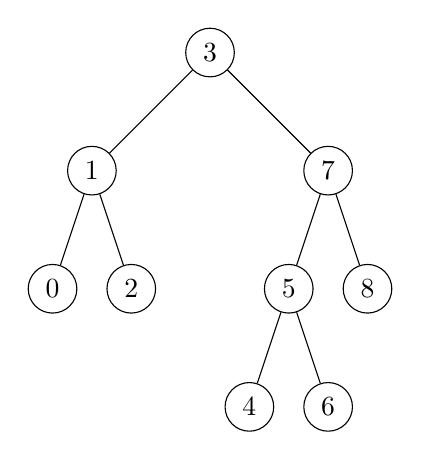
\begin{tikzpicture}
      [level 1/.style={sibling distance=30mm},
       level 2/.style={sibling distance=15mm},
       level 2/.style={sibling distance=10mm}]
      \tikzstyle{every node}=[circle,draw]
      \node{3}
      child{
        node{1}
        child{node{0}}
        child{node{2}}
      }
      child{
        node{7}
        child{
          node{5}
          child{node{4}}
          child{node{6}}
        }
        child{node{8}}
      };
    \end{tikzpicture} \hspace{4mm}
    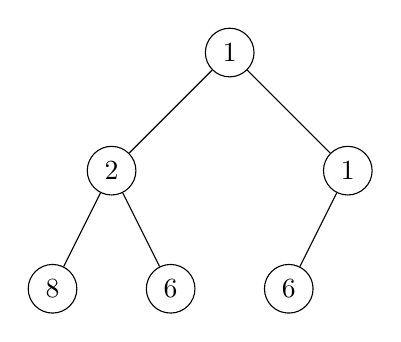
\begin{tikzpicture}
      [level 1/.style={sibling distance=30mm},
       level 2/.style={sibling distance=15mm}]
      \tikzstyle{every node}=[circle,draw]
      \node{1}
      child{
        node{2}
        child{node{8}}
        child{node{6}}
      }
      child{
        node{1}
        child{node{6}}
        child[missing]{node{k}}
      }
      ;
    \end{tikzpicture} \hspace{4mm}
    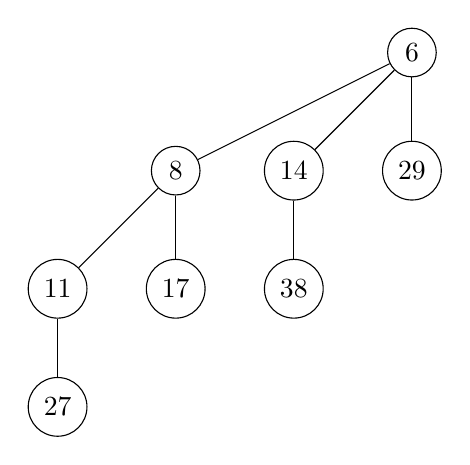
\begin{tikzpicture}[grow via three points={%
        one child at (0,-1.5) and two children at (0,-1.5) and (-1.5,-1.5)}]
      \tikzstyle{every node}=[circle,draw]
      \node at (0,0) {6}
      child{node{29}}
      child{
        node{14}
        child{
          node{38}
        }
      }
      child{
        node{8}
        child{node{17}}
        child{
          node{11}
          child{node{27}}
        }
      }
      ;
    \end{tikzpicture}
  \end{center}
  \caption{A binary search tree (on the left), a binary min-heap (in
    the middle), and a binomial tree of rank $3$ (on the right).}
  \label{fig:trees}
\end{figure}

If you are not sure whether you will stick to your current choice of
notation, then introduce a new (possibly parametric) command.  For
instance, upon
\begin{center}
  \verb|\newcommand{\Cardinality}[1]{\left\lvert#1\right\rvert}|
\end{center}
the in-lined formula \verb|$\Cardinality{S}$| typesets the cardinality
of set $S$ as $\Cardinality{S}$ with size-adjusted vertical bars and
proper spacing, but upon changing the definition of that parametric
command to
\begin{center}
  \verb|\newcommand{\Cardinality}[1]{\# #1}|
\end{center}
and recompiling, the formula \verb|$\Cardinality{S}$| typesets the
cardinality of set $S$ as $\#S$.
%
You can thus obtain an arbitrary number of changes in the document
with a \emph{constant}-time change in its source code, rather than
having to perform a \emph{linear}-time find-and-replace operation
within the source code, which is painstaking and error-prone.  The
source code of this document has some useful predefined commands about
mathematics and algorithms.

Use commands on positioning (such as \verb|\hspace|, \verb|\vspace|,
and \verb|noindent|) and appearance (such as \verb|\small| for
reducing the font size, and \verb|\textit| for italics) very
sparingly, and ideally only in (parametric) commands, as the very idea
of mark-up languages such as \LaTeX\ is to let the class designer
(usually a trained professional typesetter) decide on where things
appear and how they look.  For instance, \verb|\emph| (for emphasis)
compiles (outside italicised environments, such as \texttt{theorem})
into \textit{italics} under the \texttt{article} class used for this
document, but it may compile into \textbf{boldface} under some other
class.
\begin{center}
  Lite centrerad text bara :))
\end{center}

Note that \emph{no} absolute numbers are used in the \LaTeX\ source
code for any of the references inside this document.  For ease of
maintenance, \verb|\label| is used for giving a label to something
that is automatically numbered (such as an algorithm, equation,
figure, footnote, item, line, section, subsection, or table), and
\verb|\ref| is used for referring to a label.  An item in the
bibliography file is referred to by \verb|\cite| instead.  Upon
changing the text, it suffices to recompile, once or twice, and
possibly to run BibTeX again, in order to update all references
consistently.

Prefer \verb|Section|$\sim$\verb|\ref{sect:isort}| over
\verb|Section \ref{sect:isort}|, using the non-breaking space (given
as $\sim$) instead of the space, giving ``Section~\ref{sect:isort}''
instead of ``Section \ref{sect:isort}'' and thereby avoiding that a
cross-reference is spread across a line break, as happened in the
previous two lines: this is considered poor typesetting.

The rules of English for how many spaces to use before and after
various symbols are given in Table~\ref{tab:spacing}.  Beware that
they may be very different from the rules in your native language.

\begin{table}[t]
  \centering
  \begin{tabular}{|c|c|c|c|}
    \cline{3-4}
    \multicolumn{2}{c|}{} & \multicolumn{2}{c|}{number of spaces after} \\
    \cline{3-4}
    \multicolumn{2}{c|}{} & 0 & 1 \\
    \hline
    \multirow{2}{*}{number of spaces before} & 0 & / - & , : ; . ! ?
    ) ] \} ' '' \% \\
    \cline{2-4}
    & 1 & ( [ \{ ` `` & -- (\emph{n}-dash) --- (\emph{m}-dash) \\
    \hline
  \end{tabular}
  \caption{Spacing rules of English}
  \label{tab:spacing}
\end{table}

\vfill


\end{document}
